\documentclass[12pt, a4paper]{article}

\usepackage{fancyhdr}
\usepackage[left=4cm, right=4cm, top=4cm, bottom=4cm]{geometry}
\usepackage[utf8]{inputenc}
\usepackage[table]{xcolor}
\usepackage{amsmath}
\usepackage{enumitem}
\usepackage{graphicx}
\usepackage{hyperref}
\usepackage{geometry}
\usepackage{booktabs}
\usepackage{tikz}
\usepackage{pgfplots}
\usepackage{subcaption}
\usepackage[justification=centering]{caption}
\usepackage{floatrow}
\usepackage{xepersian}

\usetikzlibrary{arrows}
\newfloatcommand{capbtabbox}{table}[][\FBwidth]
\DeclareMathOperator{\sign}{sign}

\newcommand{\coursetitle}{شبکه‌های عصبی}
\newcommand{\doctitle}{تمرین اول}
\newcommand{\name}{محمدرضا غفرانی}
\newcommand{\studentno}{400131076}
\newcommand{\todaydate}{\today}

\settextfont{Sahel}
\setlatintextfont{Times Newer Roman}

\pagestyle{fancy}
\lhead{\textbf{\doctitle}}
\chead{\name}
\rhead{\todaydate}

\begin{document}

\begin{flushleft}
    \name \\
    \studentno \\
    \todaydate
\end{flushleft}

\begin{center}
    \huge
    \textbf{\coursetitle}
    \break
    \large
    \doctitle
\end{center}

% suppress the fancy header on the first page only
\thispagestyle{plain}

\noindent

\section*{سوال یک}

برای تولید مجموعه داده‌ای که به صورت خطی جداپذیر باشد، بدین صورت عمل می‌کنیم که دو نقطه
ثابت $\begin{bmatrix}0\\0\end{bmatrix}$ و $\begin{bmatrix}8\\8\end{bmatrix}$
را به عنوان میانگین‌های توزیع و ماتریس $\begin{bmatrix}1&0\\0&1\end{bmatrix}$ را به عنوان کواریانس
توزیع‌های گاوسی در نظر می‌گیریم. سپس برای هر کلاس تعداد ۵۰۰۰ نمونه تولید می‌کنیم.
مجموعه داده تولید شده در شکل \ref{linear_separable_dataset} دیده می‌شود.

همان‌طور که در شکل مشخص است، داده‌ها به صورت خطی جدا‌پذیر هستند، اما
برای اطمینان از وجود خطی که می‌تواند داده‌های دو کلاس را از هم جدا کند، از روش \lr{SVM} با کرنل خطی و
حاشیه سخت کمک می‌گیریم. بدین صورت که اگر با اعمال روش \lr{SVM} بر روی مجموعه دادگان به دقت
۱۰۰ درصدی برسیم، مطمئن می‌شویم که داده‌ها با استفاده از یک خط می‌توانند از هم جدا شوند.


\begin{figure}[h]
    \centering
    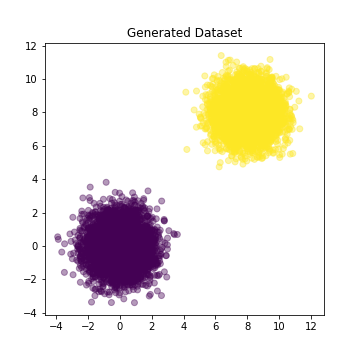
\includegraphics[scale=0.4]{images/dataset.png}
    \caption{مجموعه داده تولید شده}
    \label{linear_separable_dataset}
\end{figure}

البته می‌توان تولید مجموعه داده جداپذیر خطی را به صورت اتوماتیک نیز انجام داد.
بدین شکل که ابتدا داده‌ها را با یک مقدار‌دهی اولیه برای مقادیر میانگین و واریانس تولید کرده و سپس با استفاده
از دسته‌بند \lr{SVM} با کرنل خطی و حاشیه سخت بررسی می‌کنیم که آیا داده‌ها جداپذیر خطی هستند یا خیر. در صورتی که
داده‌ها جداپذیر خطی نبودند، فرآیند را مرتبا تکرار می‌کنیم تا به یک مجموعه دادگان جداپذیر خطی دست یابیم.

\clearpage

\section*{سوال دو}

در شکل \ref{perceptron_vs_adaline} نمونه‌ای از یک پرسپترون و واحد عصبی آدالاین دیده می‌شود.
ورودی هر دو این نورون‌ها برداری متشکل از اعداد حقیقی است. در ابتدا هر یک از درایه‌های این بردار
در یک مقدار وزن (که در ابتدا به صورت تصادفی از بازه $(0,1)$ انتخاب می‌شود)
ضرب شده و در ادامه به واحد \lr{net input} داده می‌شود. واحد \lr{net input} مجموع
حاصل‌ضرب ورودی‌ها در وزن‌های متناظر را محاسبه کرده و به واحد بعدی می‌دهد. واحد بعدی تابع فعال‌ساز نام دارد.
عملکرد این واحد بین نورون پرسپترون و آدالاین متفاوت است. در آدالاین کلاسیک از تابع همانی به عنوان تابع
فعال‌ساز استفاده می‌شود. از آن جا که خروجی تابع همانی همان ورودی آن است، بنابراین تابع فعال‌ساز در نورون آدالاین
عملا بی‌استفاده است. اما در پرسپترون نقش این واحد پررنگ است. در نورون پرسپترون از تابع فعال‌ساز $\sign(x)$
استفاده می‌شود. خروجی تابع $\sign(x)$ بدین صورت است که اگر ورودی مثبت یا صفر باشد، خروجی برابر $+1$ و در غیر این صورت
برابر $-1$ است. نورون پرسپترون تنها شامل واحد‌های بیان شده است، در حالی که نورون آدالاین علاوه بر واحد‌های
توضیح داده شده یک واحد دیگر به نام \lr{Quantizer} نیز دارد. وظیفه این تابع نگاشت مقادیر ورودی به اعداد
$+1$ و یا $-1$ است که در نتیجه مدل بتواند پیش‌بینی خود را از کلاس داده‌ها بیان کند.

در هر دو نورون آدالاین و پرسپترون خروجی تابع فعال‌ساز برای به دست آوردن خطای مدل و بهبود وزن‌ها استفاده می‌شود.
اما به دلیل این که ماهیت تابع فعال‌ساز در نورون آدالاین با پرسپترون متفاوت است بنابراین این دو نورون
روند آموزش متفاوتی دارند. از آن جا که خروجی تابع فعال‌ساز نورون آدالاین پیوسته است بنابراین می‌تواند
حتی هنگامی که خط جداکننده پیشنهادی‌اش می‌تواند داده‌ها را به درستی تفکیک کند، شیب خط جدا کننده را تغییر
دهد. این تغییر باعث می‌شود که نورون به عملکرد مناسب‌تری در حالت \lr{general} دست یابد. اما تابع فعال‌ساز
پرسپترون تنها دو خروجی $-1$ و $+1$ داشته و در نتیجه مدل تا زمانی که داده‌ها را به درستی از هم تفکیک
نمی‌کند، می‌تواند شیب خط جداکننده را تغییر دهد.

\begin{figure}[h]
    \begin{subfigure}{\linewidth}
        \centering
        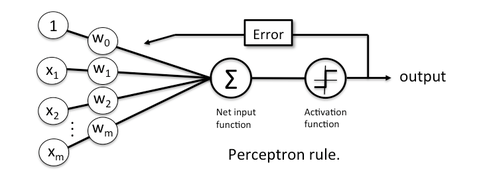
\includegraphics[width=0.6\linewidth]{images/perceptron.png}
    \end{subfigure}
    \newline
    \begin{subfigure}{\linewidth}
        \centering
        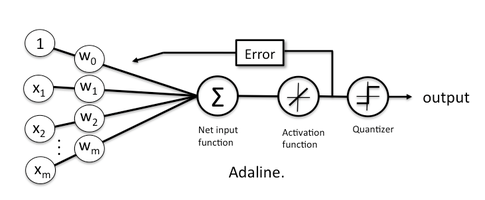
\includegraphics[width=0.6\linewidth]{images/adaline.png}
    \end{subfigure}
    \caption{مقایسه ساختار پرسپترون و آدالاین}
    \label{perceptron_vs_adaline}
\end{figure}

\clearpage

\section*{سوال سه}

ما از تابع \lr{MSE} که بر طبق اسلاید‌های درس به صورت زیر تعریف می‌شود، برای محاسبه خطا استفاده کرده‌ایم.
همچنین منظور از صحت در توضیحات زیر همان \lr{Accuracy} است.

$$\frac{1}{n}\sum_{i}(y_i - \hat{y}_i)^2$$

در ابتدا سوال را با استفاده از نورون آدالاین پاسخ می‌دهیم. برای نورون آدالاین پنج مقدار
$10^{-7}$، $10^{-6}$، $10^{-5}$، $10^{-4}$ و $10^{-3} $ را برای نرخ یادگیری بررسی کرده‌ایم.
نمودار خطا به همراه نمودار صحت عملکرد مدل بر روی داده‌های آموزشی و ارزیابی در ادامه آورده می‌شود.
با افزایش نرخ‌یادگیری سرعت حرکت مدل به سمت مینیمم سراسری افزایش می‌یابد. در نتیجه همین افزایش سرعت
مدل در طی گام‌های کم‌تری به صحت ۱۰۰درصد می‌رسد. برای مثال همان‌طور که در شکل \ref{adaline_lr_1e7}
دیده می‌شود، مدل با آموزش دیدن بر روی ۳۵ هزار داده آموزشی هنوز نتوانسته است به دقت ۸۰ درصد در
داده‌های آموزشی دست یابد در حالی که اگر نرخ یادگیری برابر $10^{-3}$ باشد (شکل \ref{adaline_lr_1e3})
مدل با دیدن 5000 داده آموزشی به صحت ۱۰۰ درصد هم بر روی داده آموزشی، هم بر روی داده ارزیابی و هم
بر روی داده آزمون می‌رسد. نتایج عملکرد مدل بر روی داده‌های آموزش و ارزیابی در هر نمودار مشخص است
اما نتایج مربوط به عملکرد بر روی داده‌های تست در قسمت پانویس هر شکل آورده شده است.

\vspace{1cm}
\begin{figure}[h]
    \begin{subfigure}{0.45\linewidth}
        \centering
        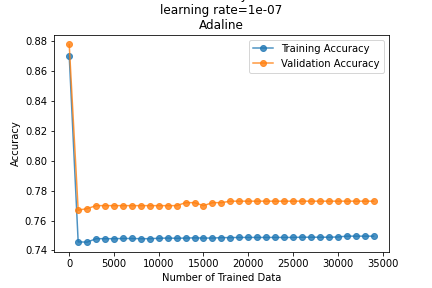
\includegraphics[width=\linewidth]{images/3/adaline/lr/acc_1e-07.png}
    \end{subfigure}
    \hfil
    \begin{subfigure}{0.45\linewidth}
        \centering
        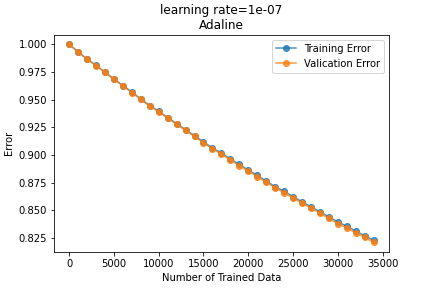
\includegraphics[width=\linewidth]{images/3/adaline/lr/error_1e-07.png}
    \end{subfigure}
    \caption{نمودار صحت عملکرد‌ و خطای مدل آدالاین با نرخ یادگیری $10^{-7}$
    \newline
    صحت نهایی مدل در داده‌های آزمون: $0.74$}
    \label{adaline_lr_1e7}
\end{figure}
\vspace{1cm}
\begin{figure}[h]
    \begin{subfigure}{0.45\linewidth}
        \centering
        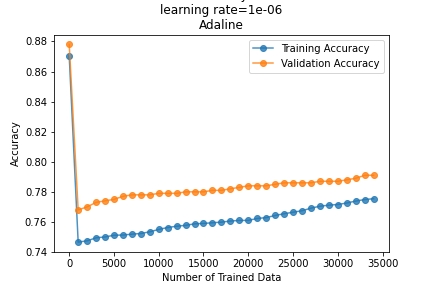
\includegraphics[width=\linewidth]{images/3/adaline/lr/acc_1e-06.png}
    \end{subfigure}
    \hfil
    \begin{subfigure}{0.45\linewidth}
        \centering
        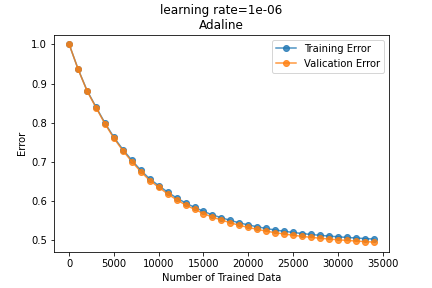
\includegraphics[width=\linewidth]{images/3/adaline/lr/error_1e-06.png}
    \end{subfigure}
    \caption{نمودار صحت عملکرد‌ و خطای مدل آدالاین با نرخ یادگیری $10^{-6}$
    \newline
    صحت نهایی مدل بر روی داده‌های آزمون: $0.77$}
\end{figure}
\begin{figure}[h]
    \begin{subfigure}{0.45\linewidth}
        \centering
        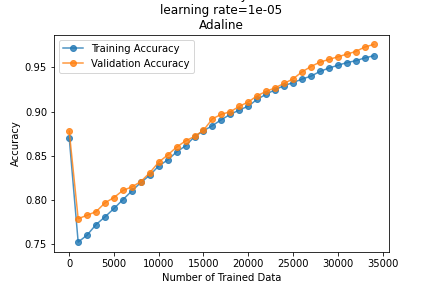
\includegraphics[width=\linewidth]{images/3/adaline/lr/acc_1e-05.png}
    \end{subfigure}
    \hfil
    \begin{subfigure}{0.45\linewidth}
        \centering
        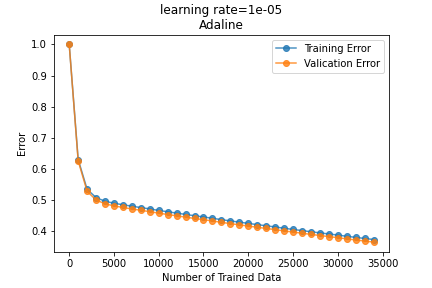
\includegraphics[width=\linewidth]{images/3/adaline/lr/error_1e-05.png}
    \end{subfigure}
    \caption{نمودار صحت عملکرد‌ و خطای مدل آدالاین با نرخ یادگیری $10^{-5}$
    \newline
    صحت نهایی مدل بر روی داده‌های آزمون: $0.97$}
\end{figure}
\begin{figure}[h]
    \begin{subfigure}{0.45\linewidth}
        \centering
        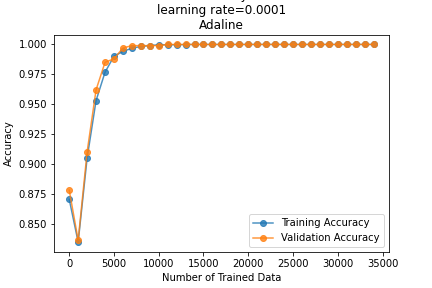
\includegraphics[width=\linewidth]{images/3/adaline/lr/acc_0.0001.png}
    \end{subfigure}
    \hfil
    \begin{subfigure}{0.45\linewidth}
        \centering
        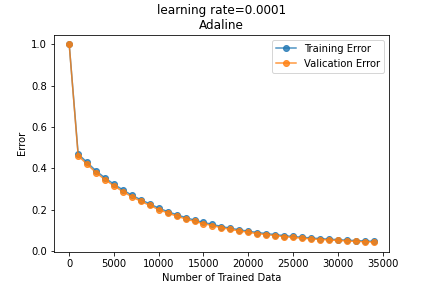
\includegraphics[width=\linewidth]{images/3/adaline/lr/error_0.0001.png}
    \end{subfigure}
    \caption{نمودار صحت عملکرد‌ و خطای مدل آدالاین با نرخ یادگیری $10^{-4}$
    \newline
    صحت نهایی مدل بر روی داده‌های آزمون: $1.0$}
\end{figure}
\clearpage
\begin{figure}[h]
    \begin{subfigure}{0.45\linewidth}
        \centering
        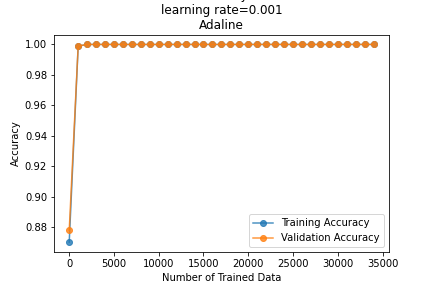
\includegraphics[width=\linewidth]{images/3/adaline/lr/acc_0.001.png}
    \end{subfigure}
    \hfil
    \begin{subfigure}{0.45\linewidth}
        \centering
        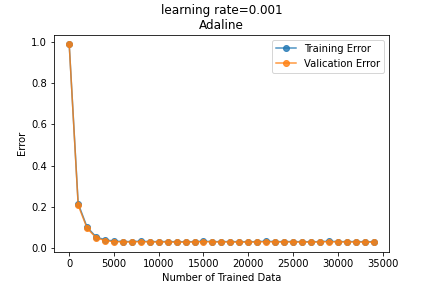
\includegraphics[width=\linewidth]{images/3/adaline/lr/error_0.001.png}
    \end{subfigure}
    \caption{نمودار صحت عملکرد‌ و خطای مدل آدالاین با نرخ یادگیری $10^{-3}$
    \newline
    صحت نهایی مدل بر روی داده‌های آزمون: $1.0$}
    \label{adaline_lr_1e3}
\end{figure}


در این قسمت می‌خواهیم تاثیر تابع فعالیت را بر عملکرد آدالاین مورد بررسی قرار دهیم.
همان‌طور که در سوال قبلی ذکر شد خروجی تابع فعال‌ساز آدالاین پیوسته بوده و همین پیوسته بودن
تابع فعال‌ساز و تاثیر‌گذار بودن این خروجی پیوسته در به روز‌رسانی وزن‌ها باعث می‌شود که این نورون
بهتر الگوی داده‌ها را کشف کند. ما در این جا از سه تابع همانی، سیگموید و $\tanh$ به عنوان تابع
فعال‌ساز نورون استفاده کرده‌ایم. در ادامه تاثیر هر یک از توابع را بر عملکرد نورون بررسی می‌کنیم.

در ابتدا نیاز است که چگونگی به‌روزرسانی وزن‌ها با استفاده از تابع فعالیت را به دست آوریم. از آن جا که
در اسلاید‌های درس روند به‌روزرسانی وزن‌ها با استفاده از تابع همانی آورده شده است، بنابراین از ذکر
مجدد آن صرف نظر می‌کنیم. می‌دانیم تابع هزینه به صورت زیر تعریف می‌شود.

\begin{eqnarray*}
    F(W) = \frac{1}{N} \sum_{i} (t_k - I_k)^2
\end{eqnarray*}

باید مشتق این تابع هزینه را محاسبه کنیم. بخشی از محاسبات که بین \lr{sigmoid} و $\tanh$ مشترک است
به صورت زیر است.

\begin{eqnarray*}
    \nabla_W F(W) & = & \nabla_W \frac{1}{N} \sum_{i} (t_k - I_k)^2 \\
    & = & \frac{1}{N} \nabla_W \sum_{i} (t_k - I_k)^2 \\
    & = & \frac{1}{N} \sum_{i} 2 \times (t_k - I_k) \nabla_W (-I_k) \\
\end{eqnarray*}

حال گرادیان جمله $I_k$ به ازای \lr{sigmoid} به صورت زیر محاسبه می‌شود.
در ادامه گرادیان نهایی به ازای این تابع فعال‌ساز نیز مشاهده می‌شود.

\begin{eqnarray*}
    \nabla_W (I_k) & = & \nabla_W \; (2 \times \sigma(W^TX)-1)\\
    & = & 2 \times \sigma(W^TX) (1-\sigma(W^TX)) \nabla_W \; (W^TX) \\
    & = & 2 \times \sigma(W^TX) (1-\sigma(W^TX)) X \\
    \nabla_W F(W) & \Longrightarrow & -4 \times \frac{1}{N} \sum_{i} (t_k - I_k) \sigma(W^TX) (1-\sigma(W^TX)) X \\
\end{eqnarray*}

حال گرادیان جمله $I_k$ را با فرض $\tanh$ محاسبه می‌کنیم. خواهیم داشت.

\begin{eqnarray*}
    \nabla_W (I_k) & = & \nabla_W \; \tanh(W^TX)\\
    & = & (1-\tanh^2(W^TX)) \nabla_W \; (W^TX) \\
    & = & (1-\tanh^2(W^TX)) X \\
    \nabla_W F(W) & \Longrightarrow & -2 \times \frac{1}{N} \sum_{i} (t_k - I_k) (1-\tanh^2(W^TX)) X \\
\end{eqnarray*}

نکته دیگری که لازم به ذکر است، این است که ما برچسب کلاس‌ها را به صورت $+1$ و $-1$ در نظر گرفته‌ایم.
از آن جا که مقادیر تابع سیگموید همواره بین $(0,1)$ است در نتیجه تابع سیگموید را به صورت
$2\times \sigma(x) - 1$ محاسبه می‌کنیم تا نتایج را به مقادیر منفی یک و مثبت یک نگاشت کند.

در ادامه روند همگرایی نورون آدالاین به ازای این توابع فعال‌ساز و نرخ یادگیری $0.001$ آورده شده است.
همان‌طور که مشاهده می‌شود هر سه تابع فعالیت توانسته‌اند به صحت ۱۰۰درصد داده‌های آموزش، ارزیابی و آزمون دست‌یابند.
تنها تفاوت آن‌ها در سرعت همگرایی است. نورون به ازای توابع فعالیت \lr{identity} و $\tanh$ بسیار سریع‌تر از
تابع فعالیت سیگموید توانسته‌اند خطا را کمینه کنند. در توجیه این رخداد می‌توان بیان کرد که
از آن جا که قدرمطلق خروجی تابع سیگموید همواره کوچک‌تر از یک است، در نتیجه با ضرب آن در باقی عبارات
از تغییرات گسترده در وزن‌ها می‌کاهد. بدین ترتیب سرعت حرکت مدل به سمت مینیمم سراسری
را کاهش می‌دهد.

\begin{figure}[!h]
    \begin{subfigure}{0.45\linewidth}
        \centering
        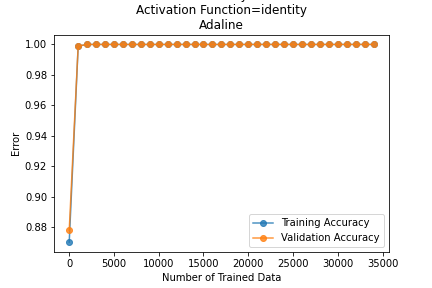
\includegraphics[width=\linewidth]{images/3/adaline/activation_func/identity_acc.png}
    \end{subfigure}
    \hfil
    \begin{subfigure}{0.45\linewidth}
        \centering
        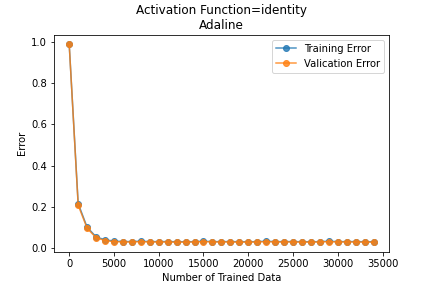
\includegraphics[width=\linewidth]{images/3/adaline/activation_func/identity_error.png}
    \end{subfigure}
    \caption{نمودار صحت عملکرد‌ و خطای مدل آدالاین با تابع فعال‌ساز همانی
    \newline
    صحت نهایی مدل بر روی داده‌های آزمون: $1.0$}
\end{figure}

\clearpage

\begin{figure}[h]
    \begin{subfigure}{0.45\linewidth}
        \centering
        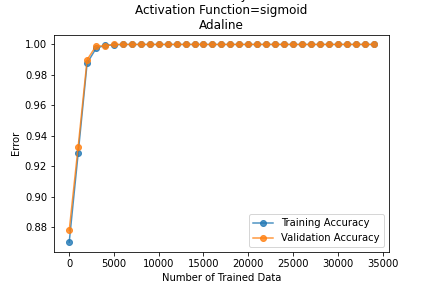
\includegraphics[width=\linewidth]{images/3/adaline/activation_func/sigmoid_acc.png}
    \end{subfigure}
    \hfil
    \begin{subfigure}{0.45\linewidth}
        \centering
        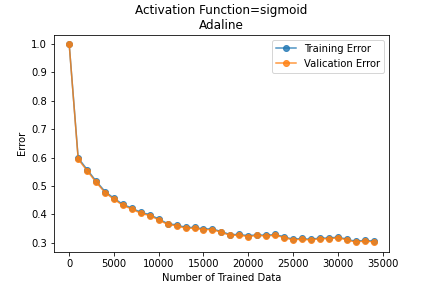
\includegraphics[width=\linewidth]{images/3/adaline/activation_func/sigmoid_error.png}
    \end{subfigure}
    \caption{نمودار صحت عملکرد‌ و خطای مدل آدالاین با تابع فعال‌ساز سیگموید
    \newline
    صحت نهایی مدل بر روی داده‌های آزمون: $1.0$}
\end{figure}
\begin{figure}[h]
    \begin{subfigure}{0.45\linewidth}
        \centering
        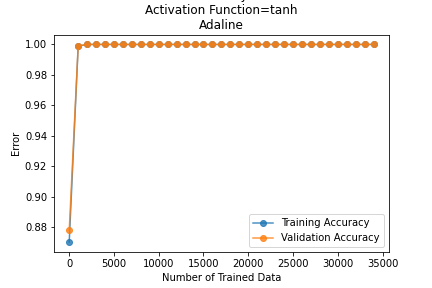
\includegraphics[width=\linewidth]{images/3/adaline/activation_func/tanh_acc.png}
    \end{subfigure}
    \hfil
    \begin{subfigure}{0.45\linewidth}
        \centering
        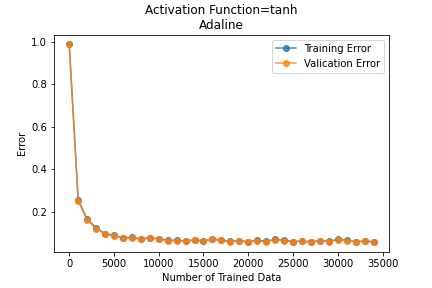
\includegraphics[width=\linewidth]{images/3/adaline/activation_func/tanh_error.png}
    \end{subfigure}
    \caption{نمودار صحت عملکرد‌ و خطای مدل آدالاین با تابع فعال‌سازی $\tanh$
    \newline
    صحت نهایی مدل بر روی داده‌های آزمون: $1.0$}
\end{figure}

حال که نتایج مربوط به نورون آدالاین بررسی شد، نتایج مربوط به نورون پرسپترون را بررسی می‌کنیم.
در ابتدا پرسپترون را با نرخ‌های یادگیری مختلف آموزش داده و تاثیر آن را بررسی می‌کنیم. مشابه حالت استفاده از
نورون آدالاین هنگامی که عدد کوچکترین را برای نرخ یادگیری در نظر می‌گیریم، نورون با سرعت کم‌تری به سمت
مینمم گرادیان حرکت کرده و در نتیجه آرام‌تر به صحت ۱۰۰ درصد می‌رسد. برای مثال هنگامی که نرخ یادگیری
برابر $0.001$ است، مدل برای رسیدن به خطای صفر نیاز است که ۵۰۰۰ داده آموزشی را ببیند در حالی که اگر
نرخ یادگیری برابر $0.1$ باشد مدل با دیدن ۱۰۰۰ داده آموزشی به خطای صفر می‌رسد. سرعت بالای حرکت به سمت
مینیمم سراسری همواره نیز نکته مثبتی برای مدل نیست چرا که ممکن است با توجه به آن که گام‌ها بلندی را
برمی‌دارد ممکن است یک مینیمم سراسری را رد کرده و در یک مینیمم محلی گیر کند. در این شکل‌ها نیز عملکرد مدل
در داده‌های آزمون در قسمت پانویس شکل‌ها آورده شده است.

\begin{figure}[h]
    \begin{subfigure}{0.45\linewidth}
        \centering
        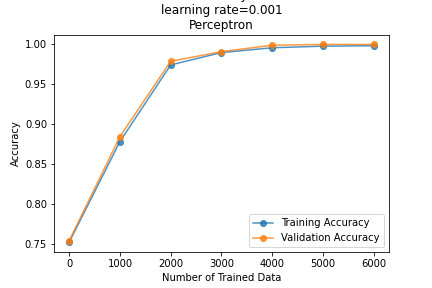
\includegraphics[width=\linewidth]{images/3/perceptron/lr/acc_0.001.png}
    \end{subfigure}
    \hfil
    \begin{subfigure}{0.45\linewidth}
        \centering
        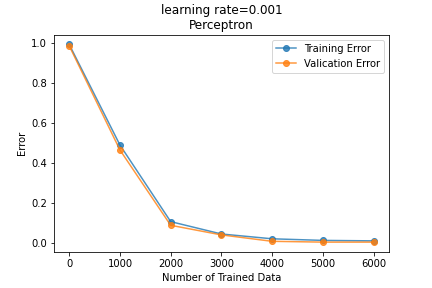
\includegraphics[width=\linewidth]{images/3/perceptron/lr/error_0.001.png}
    \end{subfigure}
    \caption{نمودار صحت عملکرد‌ و خطای مدل پرسپترون با نرخ یادگیری $10^{-3}$
    \newline
    صحت نهایی مدل در داده‌های آزمون: $0.99$}
\end{figure}
\begin{figure}[h]
    \begin{subfigure}{0.45\linewidth}
        \centering
        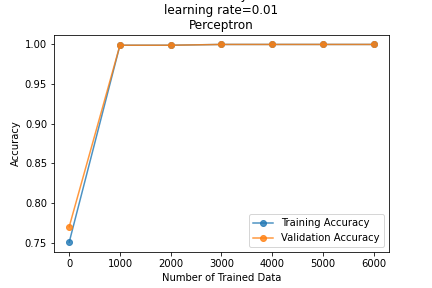
\includegraphics[width=\linewidth]{images/3/perceptron/lr/acc_0.01.png}
    \end{subfigure}
    \hfil
    \begin{subfigure}{0.45\linewidth}
        \centering
        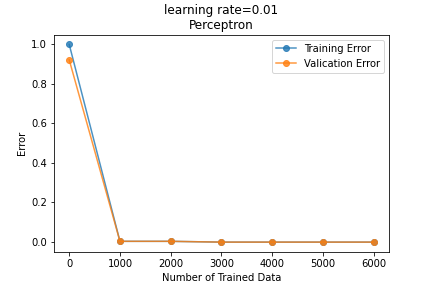
\includegraphics[width=\linewidth]{images/3/perceptron/lr/error_0.01.png}
    \end{subfigure}
    \caption{نمودار صحت عملکرد‌ و خطای مدل پرسپترون با نرخ یادگیری $10^{-2}$
    \newline
    صحت نهایی مدل بر روی داده‌های آزمون: $1.0$}
\end{figure}
\begin{figure}[h]
    \begin{subfigure}{0.45\linewidth}
        \centering
        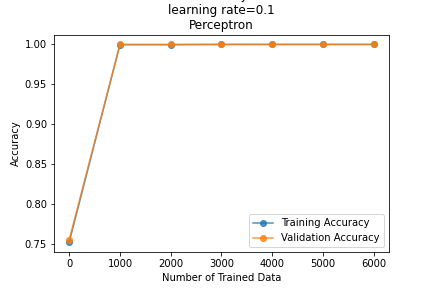
\includegraphics[width=\linewidth]{images/3/perceptron/lr/acc_0.1.png}
    \end{subfigure}
    \hfil
    \begin{subfigure}{0.45\linewidth}
        \centering
        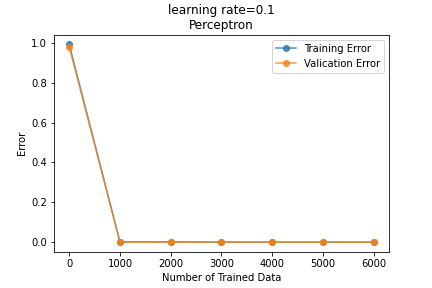
\includegraphics[width=\linewidth]{images/3/perceptron/lr/error_0.1.png}
    \end{subfigure}
    \caption{نمودار صحت عملکرد‌ و خطای مدل پرسپترون با نرخ یادگیری $0.1$
    \newline
    صحت نهایی مدل بر روی داده‌های آزمون: $1.0$}
\end{figure}

\clearpage

\begin{figure}[h]
    \begin{subfigure}{0.45\linewidth}
        \centering
        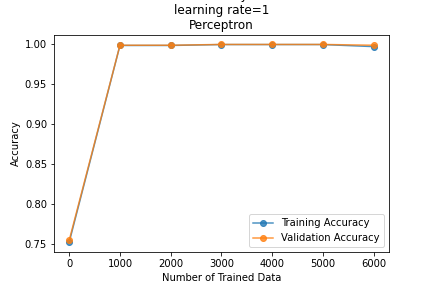
\includegraphics[width=\linewidth]{images/3/perceptron/lr/acc_1.png}
    \end{subfigure}
    \hfil
    \begin{subfigure}{0.45\linewidth}
        \centering
        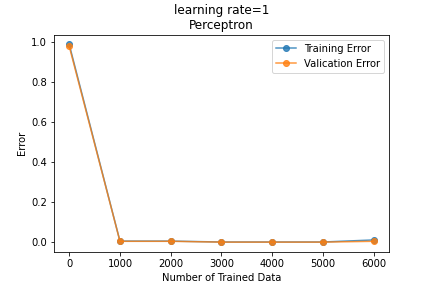
\includegraphics[width=\linewidth]{images/3/perceptron/lr/error_1.png}
    \end{subfigure}
    \caption{نمودار صحت عملکرد‌ و خطای مدل پرسپترون با نرخ یادگیری $1$
    \newline
    صحت نهایی مدل بر روی داده‌های آزمون: $1.0$}
\end{figure}

\begin{figure}[h]
    \begin{subfigure}{0.45\linewidth}
        \centering
        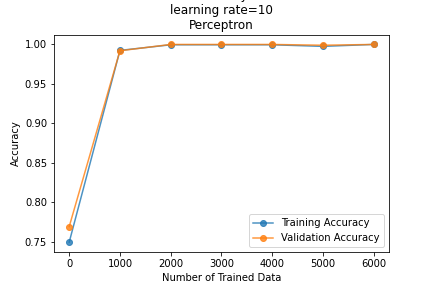
\includegraphics[width=\linewidth]{images/3/perceptron/lr/acc_10.png}
    \end{subfigure}
    \hfil
    \begin{subfigure}{0.45\linewidth}
        \centering
        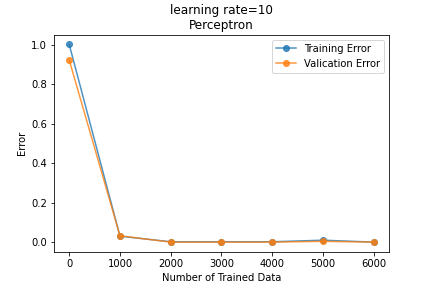
\includegraphics[width=\linewidth]{images/3/perceptron/lr/error_10.png}
    \end{subfigure}
    \caption{نمودار صحت عملکرد‌ و خطای مدل پرسپترون با نرخ یادگیری $10$
    \newline
    صحت نهایی مدل بر روی داده‌های آزمون: $1.0$}
\end{figure}

در نهایت قصد داریم تاثیر تابع فعال‌ساز را بر عملکرد پرسپترون مورد بررسی قرار دهیم.
از آن جا که خروجی تابع فعالیت پرسپترون یکی از دو مقدار $-1$ یا $+1$ است بنابراین
گستره انتخاب وسیعی برای این تابع وجود ندارد. ما در این جا از همان تابع $\sign$ استفاده می‌کنیم،
با این تفاوت که مقداری را به عنوان \lr{offset} برای تابع در نظر گرفته و در واقع از تابع $\sign(x-\text{\lr{offset}})$
استفاده می‌کنیم. سه مقدار مختلف را برای \lr{offset} بررسی می‌کنیم. برای آن که نتایج قابل
واضح‌تر باشد، نرخ‌یادگیری را برابر $0.0001$ در نظر می‌گیریم. نتایج حاصل از این آزمایش در شکل‌های زیر قابل مشاهده
است. همان‌طور که مشاهده می‌شود شیب یادگیری مدل با استفاده از توابع فعال‌ساز $\sign(x-5)$، $\sign(x)$ و $\sign(x+5)$
چندان تفاوت نکرده است. دقت شود که مقیاس محور عمودی در نمودار‌های مختلف متفاوت است. علت این کار را می‌توان یکسان
بودن مشتق این توابع فعالیت دانست. تاثیر مقدار \lr{offset} به صورت بایاس بوده و تنها نمودار‌ها را به سمت
راست و چپ شیفت داده است. به همین دلیل است که پرسپترون با تابع فعالیت $\sign(x+5)$ از همان ابتدا دارای صحت
100 درصد بوده در حالی که پرسپترونی که از تابع فعالیت $\sign(x-5)$ استفاده می‌کند اندکی طول می‌کشد تا به صحت 100
دست پیدا کند. در نهایت هر سه پرسپترون توانسته‌اند به صحت ۱۰۰ درصد بر روی داده‌های آموزشی و
ارزیابی و نزدیک به ۱۰۰ در داده آزمون دست یابند.

\begin{figure}[h]
    \begin{subfigure}{0.45\linewidth}
        \centering
        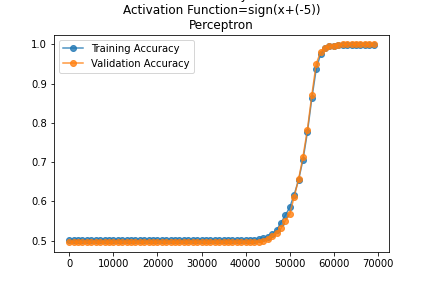
\includegraphics[width=\linewidth]{images/3/perceptron/activation_func/5.png}
    \end{subfigure}
    \hfil
    \begin{subfigure}{0.45\linewidth}
        \centering
        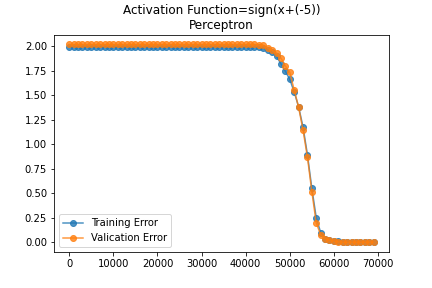
\includegraphics[width=\linewidth]{images/3/perceptron/activation_func/6.png}
    \end{subfigure}
    \caption{نمودار صحت عملکرد‌ و خطای پرسپترون با تابع فعال‌ساز $\sign(x-5)$
    \newline
    صحت نهایی مدل بر روی داده‌های آزمون: $1.0$}
\end{figure}
\begin{figure}[h]
    \begin{subfigure}{0.45\linewidth}
        \centering
        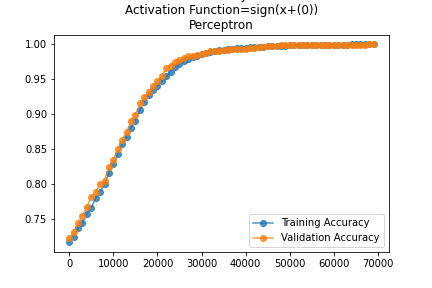
\includegraphics[width=\linewidth]{images/3/perceptron/activation_func/1.png}
    \end{subfigure}
    \hfil
    \begin{subfigure}{0.45\linewidth}
        \centering
        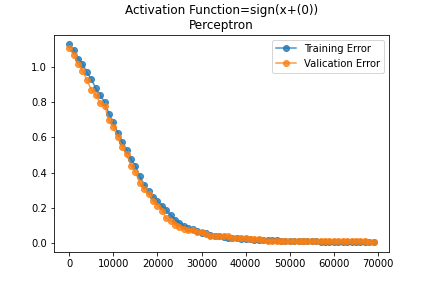
\includegraphics[width=\linewidth]{images/3/perceptron/activation_func/2.png}
    \end{subfigure}
    \caption{نمودار صحت عملکرد‌ و خطای پرسپترون با تابع فعال‌ساز $\sign(x)$
    \newline
    صحت نهایی مدل بر روی داده‌های آزمون: $0.99$}
\end{figure}
\begin{figure}[h]
    \begin{subfigure}{0.45\linewidth}
        \centering
        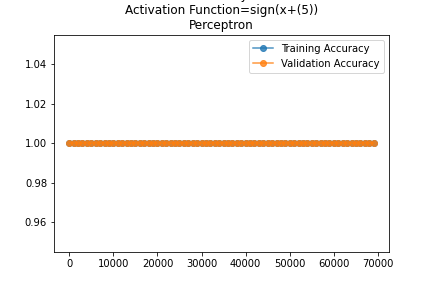
\includegraphics[width=\linewidth]{images/3/perceptron/activation_func/3.png}
    \end{subfigure}
    \hfil
    \begin{subfigure}{0.45\linewidth}
        \centering
        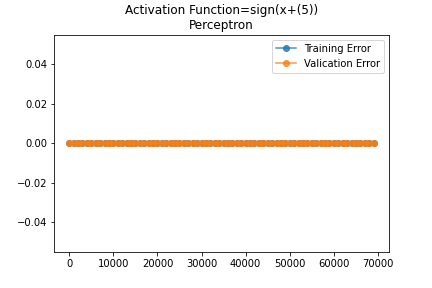
\includegraphics[width=\linewidth]{images/3/perceptron/activation_func/4.png}
    \end{subfigure}
    \caption{نمودار صحت عملکرد‌ و خطای پرسپترون با تابع فعال‌ساز $\sign(x+5)$
    \newline
    صحت نهایی مدل بر روی داده‌های آزمون: $1.0$}
\end{figure}

\clearpage

در نهایت عملکرد کلی دو نورون آدالاین و پرسپترون را با هم مقایسه می‌کنیم.
طبق نتایجی که تا به الان به دست آمد تفاوت چندانی بین عملکرد نورون و پرسپترون بر روی داده‌های آموزش، ارزیابی
و تست مشاهده نمی‌شود و هر دو این نورون‌ها می‌توانند با تنظیم بهینه پارامتر‌ها به صحت ۱۰۰ دست یابند. اما نکته
مهمی که وجود دارد خط جداکننده نهایی است که این دو مدل به آن دست یافته‌اند. در شکل \ref{perceptron_adaline_comparison}
خط جداکننده‌ای که این دو مدل در طی ۱۰ گام یادگیری رسیده‌اند مشاهده می‌شود. برای به دست آوردن
این خط جداکننده از تابع فعالیت نورون آدالاین را تابع همانی در نظر گرفته و مقدار نرخ یادگیری را برابر $0.001$
فرض کرده‌ایم. برای نورون پرسپترون نیز نرخ یادگیری را برابر $0.01$ و تابع فعال‌ساز را تابع $\sign(x)$ در نظر گرفته‌ایم.
در آزمایش‌های قبل هر یک از نورون‌ها با استفاده از این پارامتر‌ها به بهترین نتایج رسیده بودند.

همان‌طور که در شکل \ref{perceptron_adaline_comparison} دیده می‌شود، خط جداکننده آدالاین الگوی داده‌ها را
بهتر توانسته‌ است متوجه شود. در حالی که خط جداکننده پرسپترون صرفا تلاش کرده است داده‌های فعلی را از هم
جدا کند.

\vspace{.5cm}

\begin{figure}[h]
    \begin{subfigure}{0.45\linewidth}
        \centering
        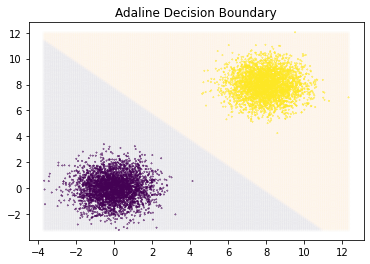
\includegraphics[width=\linewidth]{images/3/adaline.png}
    \end{subfigure}
    \begin{subfigure}{0.45\linewidth}
        \centering
        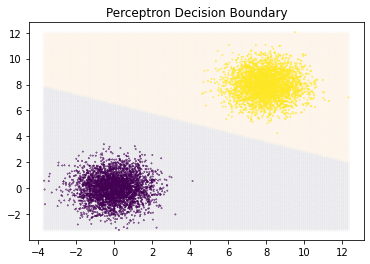
\includegraphics[width=\linewidth]{images/3/perceptron.png}
    \end{subfigure}
    \caption{مقایسه خط جداکننده پرسپترون و آدالاین}
    \label{perceptron_adaline_comparison}
\end{figure}

\vspace{0.5cm}

دلیل دیگری که باعث برتری نورون آدالاین به نورون پرسپترون می‌شود، به‌روزرسانی خط جداکننده
حتی زمانی که مدل می‌تواند تمامی داده‌ها را به درستی برچسب بزند است. بدین طریق آدالاین می‌تواند با درک بهتر از
الگوی داده‌ها، جداکننده مناسب‌تری را پیشنهاد دهد. با توجه به این دلایل ما مدل آدالاین را بهتر از مدل پرسپترون
می‌دانیم.

\clearpage

\section*{سوال چهار}

برای این قسمت نیز مشابه سوال ۲ از نقاط ثابت $\begin{bmatrix}0\\0\end{bmatrix}$، $\begin{bmatrix}0\\10\end{bmatrix}$،
$\begin{bmatrix}10\\0\end{bmatrix}$ و $\begin{bmatrix}10\\10\end{bmatrix}$ به عنوان مراکز توزیع گاوسی با کواریانس
$I=\begin{bmatrix}1&0\\0&1\end{bmatrix}$ استفاده می‌کنیم. در شکل \ref{xor_dataset} نمودار داده‌ها رسم شده است.
در این شکل به وضوح مشخص است که داده‌ها به صورت خطی جداپذیر نیستند و در نتیجه آزمایشی برای بررسی جداپذیر بودن
داده‌ها انجام نمی‌دهیم.

\begin{figure}[h]
    \centering
    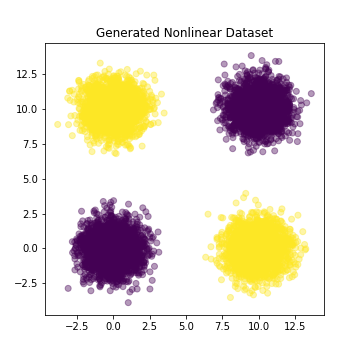
\includegraphics[scale=0.5]{images/nonlinear_dataset.png}
    \caption{داده‌های جداناپذیر خطی تولید شده}
    \label{xor_dataset}
\end{figure}

\clearpage

\section*{سوال پنجم}

ابتدا تاثیر نرخ یادگیری را بر روی عملکرد نورون آدالاین و مجموعه داده غیرخطی
بررسی می‌کنیم. در ادامه نتایج مربوط به عملکرد نورون آدالاین با تغییر نرخ یادگیری آورده شده است.
همان‌طور که مشاهده می‌شود هنگامی که نرخ یادگیری عدد بزرگ‌تری است، مدل نوسانات زیادی داشته و مدام
بین مقادیر بالا و پایین می‌جهد. با توجه به این مورد نمی‌توان قضاوتی در رابطه با تاثیر نرخ‌های یادگیری مختلف
داد. البته با توجه به خطی بودن جداکننده نمی‌توان انتظار رسیدن به صحت بالای ۷۵ درصد را داشت.

در شکل \ref{lkm} به نظر می‌رسد که خطای عملکرد مدل به صفر رسیده است. با بررسی دقیق مقادیر
حاصل شده از عملکرد این مدل مشخص شد که این مورد به دلیل نوع رسم کتابخانه \lr{matplotlib}
بوده و با توجه به آن که مقادیر بسیار نزدیک به ۱ بوده‌اند، یک را در قسمت بالای سمت چپ نمودار
نوشته و از باقی مقادیر کم کرده است.

\vspace{1cm}
\begin{figure}[h]
    \begin{subfigure}{0.45\linewidth}
        \centering
        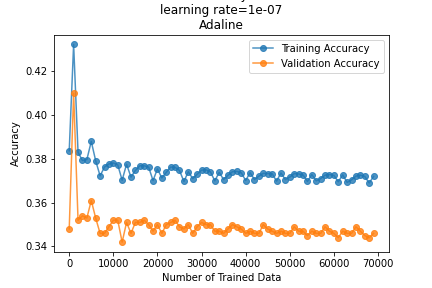
\includegraphics[width=\linewidth]{images/5/adaline/lr/acc_1e-07.png}
    \end{subfigure}
    \hfil
    \begin{subfigure}{0.45\linewidth}
        \centering
        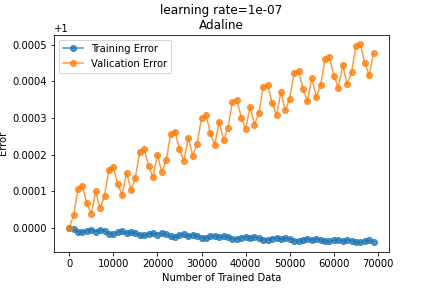
\includegraphics[width=\linewidth]{images/5/adaline/lr/error_1e-07.png}
    \end{subfigure}
    \caption{نمودار صحت عملکرد‌ و خطای مدل آدالاین با نرخ یادگیری $10^{-7}$
    \newline
    صحت نهایی مدل در داده‌های آزمون: $0.37$}
    \label{lkm}
\end{figure}
\vspace{1cm}
\begin{figure}[h]
    \begin{subfigure}{0.45\linewidth}
        \centering
        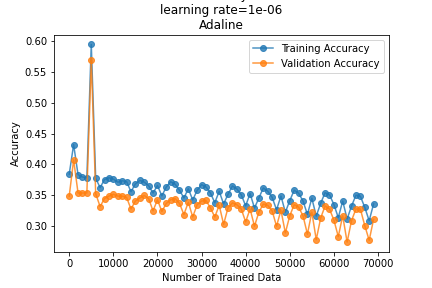
\includegraphics[width=\linewidth]{images/5/adaline/lr/acc_1e-06.png}
    \end{subfigure}
    \hfil
    \begin{subfigure}{0.45\linewidth}
        \centering
        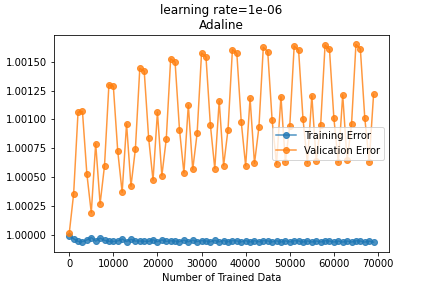
\includegraphics[width=\linewidth]{images/5/adaline/lr/error_1e-06.png}
    \end{subfigure}
    \caption{نمودار صحت عملکرد‌ و خطای مدل آدالاین با نرخ یادگیری $10^{-6}$
    \newline
    صحت نهایی مدل بر روی داده‌های آزمون: $0.31$}
\end{figure}
\begin{figure}[h]
    \begin{subfigure}{0.45\linewidth}
        \centering
        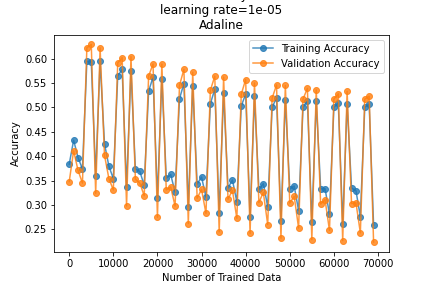
\includegraphics[width=\linewidth]{images/5/adaline/lr/acc_1e-05.png}
    \end{subfigure}
    \hfil
    \begin{subfigure}{0.45\linewidth}
        \centering
        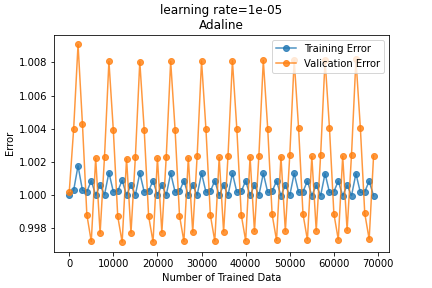
\includegraphics[width=\linewidth]{images/5/adaline/lr/error_1e-05.png}
    \end{subfigure}
    \caption{نمودار صحت عملکرد‌ و خطای مدل آدالاین با نرخ یادگیری $10^{-5}$
    \newline
    صحت نهایی مدل بر روی داده‌های آزمون: $0.49$}
\end{figure}
\begin{figure}[h]
    \begin{subfigure}{0.45\linewidth}
        \centering
        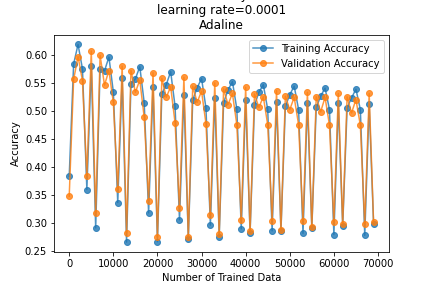
\includegraphics[width=\linewidth]{images/5/adaline/lr/acc_0.0001.png}
    \end{subfigure}
    \hfil
    \begin{subfigure}{0.45\linewidth}
        \centering
        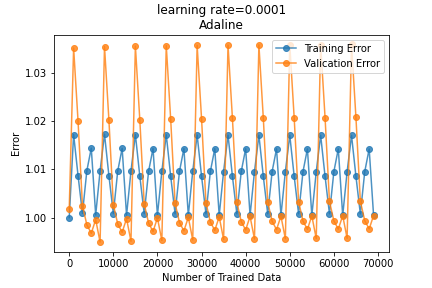
\includegraphics[width=\linewidth]{images/5/adaline/lr/error_0.0001.png}
    \end{subfigure}
    \caption{نمودار صحت عملکرد‌ و خطای مدل آدالاین با نرخ یادگیری $10^{-4}$
    \newline
    صحت نهایی مدل بر روی داده‌های آزمون: $0.50$}
\end{figure}
\begin{figure}[h]
    \begin{subfigure}{0.45\linewidth}
        \centering
        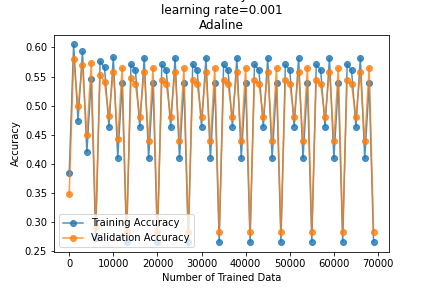
\includegraphics[width=\linewidth]{images/5/adaline/lr/acc_0.001.png}
    \end{subfigure}
    \hfil
    \begin{subfigure}{0.45\linewidth}
        \centering
        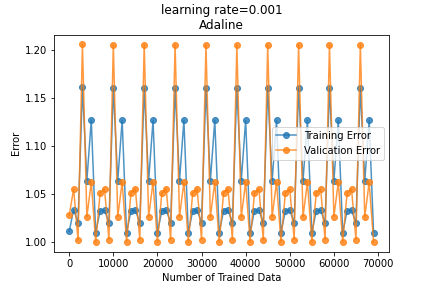
\includegraphics[width=\linewidth]{images/5/adaline/lr/error_0.001.png}
    \end{subfigure}
    \caption{نمودار صحت عملکرد‌ و خطای مدل آدالاین با نرخ یادگیری $10^{-3}$
    \newline
    صحت نهایی مدل بر روی داده‌های آزمون: $0.34$}
\end{figure}

\clearpage

در ادامه تابع فعال‌ساز آدالاین را تغییر داده و تاثیر آن را بررسی می‌کنیم. در این حالت نرخ یادگیری را برابر
$0.001$ در نظر گرفته‌ایم. از تکرار محاسبات مربوط به به‌روزرسانی وزن‌ها نیز با توجه به آن که در توضیحات
سوال سه آورده بودیم، صرف نظر کرده‌ایم.

با صرف نگاه کردن به نتایج عملکرد مدل بر روی داده‌های آزمون، به نظر می‌رسد عملکرد مدل با استفاده از
تابع فعال‌ساز $\tanh$ نسبت به دیگر توابع بهتر است. اما با توجه به نوسانات موجود در نمودار‌ خطای
آموزش و ارزیابی مشخص می‌شود که این عملکرد مناسب اتفاقی بوده و صرفا به این دلیل است که مدل هنگامی که در
بهترین حالت خود بوده، آموزش قطع شده است. بنابراین در این حالت نیز بهترین یا بدترین عملکردی وجود نداشته
و همه عملکرد‌ها تقریبا یکسان هستند.

\vspace{1cm}

\begin{figure}[h]
    \begin{subfigure}{0.45\linewidth}
        \centering
        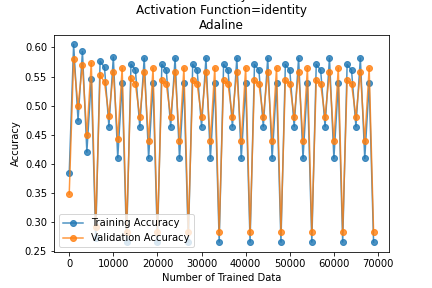
\includegraphics[width=\linewidth]{images/5/adaline/activation_func/identity_acc.png}
    \end{subfigure}
    \hfil
    \begin{subfigure}{0.45\linewidth}
        \centering
        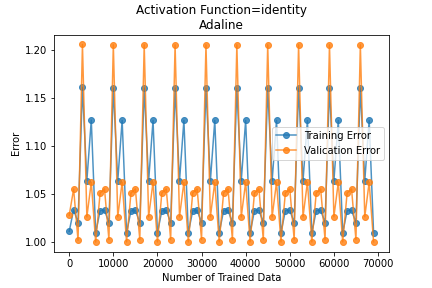
\includegraphics[width=\linewidth]{images/5/adaline/activation_func/identity_error.png}
    \end{subfigure}
    \caption{نمودار صحت عملکرد‌ و خطای مدل آدالاین با تابع فعال‌ساز همانی
    \newline
    صحت نهایی مدل بر روی داده‌های آزمون: $0.34$}
\end{figure}

\vspace{1cm}

\begin{figure}[h]
    \begin{subfigure}{0.45\linewidth}
        \centering
        \includegraphics[width=\linewidth]{images/5/adaline/activation_func/sigmoid_acc.png}
    \end{subfigure}
    \hfil
    \begin{subfigure}{0.45\linewidth}
        \centering
        \includegraphics[width=\linewidth]{images/5/adaline/activation_func/sigmoid_error.png}
    \end{subfigure}
    \caption{نمودار صحت عملکرد‌ و خطای مدل آدالاین با تابع فعال‌ساز سیگموید
    \newline
    صحت نهایی مدل بر روی داده‌های آزمون: $0.51$}
\end{figure}

\clearpage

\begin{figure}[h]
    \begin{subfigure}{0.45\linewidth}
        \centering
        \includegraphics[width=\linewidth]{images/5/adaline/activation_func/tanh_acc.png}
    \end{subfigure}
    \hfil
    \begin{subfigure}{0.45\linewidth}
        \centering
        \includegraphics[width=\linewidth]{images/5/adaline/activation_func/tanh_error.png}
    \end{subfigure}
    \caption{نمودار صحت عملکرد‌ و خطای مدل آدالاین با تابع فعال‌سازی $\tanh$
    \newline
    صحت نهایی مدل بر روی داده‌های آزمون: $0.59$}
\end{figure}

\vspace{1cm}

در ادامه تاثیر نرخ یادگیری را بر روی مدل پرسپترون و در مجموعه داده جداناپذیر خطی بررسی می‌کنیم.
همان‌طور که در ادامه مشاهده می‌شود، مدل پرسپترون مشابه مدل آدالاین روی مجموعه داده آموزشی نوسانات
زیادی داشته و در نتیجه نتایج به دست آورده قابل اتکا نیستند. بعلاوه هیچ یک از مدل‌ها نتوانسته است
به صحت خوبی روی مجموعه آزمون دست یابد. تنها تفاوتی که به ازای نرخ‌های یادگیری مختلف مشاهده می‌شود، دامنه
زیاد نوسانات به ازای نرخ‌های یادگیری بالا و کم بودن این دامنه نوسانات به ازای نرخ‌ها یادگیری پایین است.

\vspace{1cm}

\begin{figure}[h]
    \begin{subfigure}{0.45\linewidth}
        \centering
        \includegraphics[width=\linewidth]{images/5/perceptron/lr/acc_0.001.png}
    \end{subfigure}
    \hfil
    \begin{subfigure}{0.45\linewidth}
        \centering
        \includegraphics[width=\linewidth]{images/5/perceptron/lr/error_0.001.png}
    \end{subfigure}
    \caption{نمودار صحت عملکرد‌ و خطای مدل پرسپترون با نرخ یادگیری $10^{-3}$
    \newline
    صحت نهایی مدل در داده‌های آزمون: $0.58$}
\end{figure}
\begin{figure}[h]
    \begin{subfigure}{0.45\linewidth}
        \centering
        \includegraphics[width=\linewidth]{images/5/perceptron/lr/acc_0.01.png}
    \end{subfigure}
    \hfil
    \begin{subfigure}{0.45\linewidth}
        \centering
        \includegraphics[width=\linewidth]{images/5/perceptron/lr/error_0.01.png}
    \end{subfigure}
    \caption{نمودار صحت عملکرد‌ و خطای مدل پرسپترون با نرخ یادگیری $10^{-2}$
    \newline
    صحت نهایی مدل بر روی داده‌های آزمون: $0.51$}
\end{figure}
\begin{figure}[h]
    \begin{subfigure}{0.45\linewidth}
        \centering
        \includegraphics[width=\linewidth]{images/5/perceptron/lr/acc_0.1.png}
    \end{subfigure}
    \hfil
    \begin{subfigure}{0.45\linewidth}
        \centering
        \includegraphics[width=\linewidth]{images/5/perceptron/lr/error_0.1.png}
    \end{subfigure}
    \caption{نمودار صحت عملکرد‌ و خطای مدل پرسپترون با نرخ یادگیری $0.1$
    \newline
    صحت نهایی مدل بر روی داده‌های آزمون: $0.59$}
\end{figure}
\begin{figure}[h]
    \begin{subfigure}{0.45\linewidth}
        \centering
        \includegraphics[width=\linewidth]{images/5/perceptron/lr/acc_1.png}
    \end{subfigure}
    \hfil
    \begin{subfigure}{0.45\linewidth}
        \centering
        \includegraphics[width=\linewidth]{images/5/perceptron/lr/error_1.png}
    \end{subfigure}
    \caption{نمودار صحت عملکرد‌ و خطای مدل پرسپترون با نرخ یادگیری $1$
    \newline
    صحت نهایی مدل بر روی داده‌های آزمون: $0.60$}
\end{figure}
\clearpage
\begin{figure}[h]
    \begin{subfigure}{0.45\linewidth}
        \centering
        \includegraphics[width=\linewidth]{images/5/perceptron/lr/acc_10.png}
    \end{subfigure}
    \hfil
    \begin{subfigure}{0.45\linewidth}
        \centering
        \includegraphics[width=\linewidth]{images/5/perceptron/lr/error_10.png}
    \end{subfigure}
    \caption{نمودار صحت عملکرد‌ و خطای مدل پرسپترون با نرخ یادگیری $10$
    \newline
    صحت نهایی مدل بر روی داده‌های آزمون: $0.58$}
\end{figure}

در نهایت سعی می‌کنیم با تغییر تابع فعال‌ساز پرسپترون داده‌ها را از هم تفکیک کنیم.
شکل‌های مربوط به عملکرد این مدل در صفحه بعد آورده شده است.
در این حالت نیز به علت بالا بودن دامنه نوسانات نمی‌توان یکی از مدل‌ها را به عنوان بهترین عملکرد برگزید.
اما در کل مدل به صحت مناسبی بر روی داده‌های تست دست‌ یافته است.

جمع‌بندی این که نورون مرتبه یک آدالاین و پرسپترون تلاش می‌کنند داده‌ها را با استفاده از یک خط
جدا کنند. اگر مجموعه داده به صورت خطی جداپذیر باشد، در این صورت هر دو این نورون‌ها می‌توانند
داده‌ها را به درستی از هم تفکیک کنند، در غیر این صورت در هنگام آموزش مدل بسیار نوسان کرده و نمی‌توانند
به جمع‌بندی برسند. در این حالت عملکرد مدل نیز قابل اتکا نیست، چرا که معمولا در هنگامی که مدل بهترین
عملکرد را داشته، آموزش متوقف شده و در نتیجه مدل توانسته به نتیجه خوبی برسد.

\clearpage

\begin{figure}[h]
    \begin{subfigure}{0.45\linewidth}
        \centering
        \includegraphics[width=\linewidth]{images/5/perceptron/activation_func/5.png}
    \end{subfigure}
    \hfil
    \begin{subfigure}{0.45\linewidth}
        \centering
        \includegraphics[width=\linewidth]{images/5/perceptron/activation_func/6.png}
    \end{subfigure}
    \caption{نمودار صحت عملکرد‌ و خطای پرسپترون با تابع فعال‌ساز $\sign(x-5)$
    \newline
    صحت نهایی مدل بر روی داده‌های آزمون: $0.60$}
\end{figure}
\begin{figure}[h]
    \begin{subfigure}{0.45\linewidth}
        \centering
        \includegraphics[width=\linewidth]{images/5/perceptron/activation_func/1.png}
    \end{subfigure}
    \hfil
    \begin{subfigure}{0.45\linewidth}
        \centering
        \includegraphics[width=\linewidth]{images/5/perceptron/activation_func/2.png}
    \end{subfigure}
    \caption{نمودار صحت عملکرد‌ و خطای پرسپترون با تابع فعال‌ساز $\sign(x)$
    \newline
    صحت نهایی مدل بر روی داده‌های آزمون: $0.58$}
\end{figure}
\begin{figure}[!h]
    \begin{subfigure}{0.45\linewidth}
        \centering
        \includegraphics[width=\linewidth]{images/5/perceptron/activation_func/3.png}
    \end{subfigure}
    \hfil
    \begin{subfigure}{0.45\linewidth}
        \centering
        \includegraphics[width=\linewidth]{images/5/perceptron/activation_func/4.png}
    \end{subfigure}
    \caption{نمودار صحت عملکرد‌ و خطای پرسپترون با تابع فعال‌ساز $\sign(x+5)$
    \newline
    صحت نهایی مدل بر روی داده‌های آزمون: $0.58$}
\end{figure}

\clearpage

\section*{سوال ششم}

ابتدا تاثیر نرخ یادگیری را بر روی عملکرد نورون آدالاین درجه دو در مجموعه داده غیرخطی
را بررسی می‌کنیم. همان‌طور که در شکل‌های زیر مشاهده می‌شود، روند کلی آموزش خوب بوده و
برخلاف نورون آدالاین درجه یک که در آن نوسانات زیادی در زمان آموزش دیده می‌شد، در زمان
آموزش این مدل نوسان آنچنانی در روند آموزش دیده نمی‌شود. علت این کار دخیل کردن جمله‌های درجه‌ دو
و حاصل‌ضرب جمله‌ها در ورودی مدل است. ما در این جا از مدل آدالاین با ورودی زیر استفاده می‌کنیم.
این مدل همان مدل موجود در اسلاید‌های درس است.

$$(1, x_1, x_2, x_1^2, x_2^2, x_1 x_2)$$

از بین مدل با نرخ‌های یادگیری زیر تنها مدل‌هایی که با نرخ یادگیری $10^{-5}$ و $10^{-6}$
آموزش دیده‌اند، توانسته‌اند به صحت بالای 90 درصد برسند. البته این جمله به این معنا نیست که
صحت ارائه شده توسط دیگر مدل‌ها قابل قبول نیست. ما امیدوار بودیم که همه مدل‌ها با طی ۵۰گام
بتوانند به خوبی تمامی داده‌ها را از هم تفکیک کنند، اما به نظر می‌رسد بعضی از مدل‌ها نیاز به
گام‌های بیشتری برای کامل‌کردن یادگیری نیاز داشتند. بعضی دیگر از مدل‌ها نظیر مدل با نرخ یادگیری
$10^{-7}$ نیز به نظر می‌رسد که در مینیمم محلی به همگرایی رسیده باشند. با توجه به شکل‌ها
و توضیحات به این نتیجه می‌رسیم که هنگامی که نرخ یادگیری کم است
مدل با سرعت کم‌تری به سمت مینیمم حرکت می‌کند، در نتیجه این به تعداد گام بیشتری نیاز است
تا بتواند عملکرد قابل قبولی را ارائه دهد.

\vspace{1cm}

\begin{figure}[h]
    \begin{subfigure}{0.45\linewidth}
        \centering
        \includegraphics[width=\linewidth]{images/6/adaline/lr/acc_1e-09.png}
    \end{subfigure}
    \hfil
    \begin{subfigure}{0.45\linewidth}
        \centering
        \includegraphics[width=\linewidth]{images/6/adaline/lr/error_1e-09.png}
    \end{subfigure}
    \caption{نمودار صحت عملکرد‌ و خطای آدالاین درجه ۲ با نرخ یادگیری $10^{-9}$
    \newline
    صحت نهایی مدل در داده‌های آزمون: $0.82$}
\end{figure}
\begin{figure}[h]
    \begin{subfigure}{0.45\linewidth}
        \centering
        \includegraphics[width=\linewidth]{images/6/adaline/lr/acc_1e-08.png}
    \end{subfigure}
    \hfil
    \begin{subfigure}{0.45\linewidth}
        \centering
        \includegraphics[width=\linewidth]{images/6/adaline/lr/error_1e-08.png}
    \end{subfigure}
    \caption{نمودار صحت عملکرد‌ و خطای آدالاین درجه ۲ با نرخ یادگیری $10^{-8}$
    \newline
    صحت نهایی مدل در داده‌های آزمون: $0.82$}
\end{figure}
\begin{figure}[h]
    \begin{subfigure}{0.45\linewidth}
        \centering
        \includegraphics[width=\linewidth]{images/6/adaline/lr/acc_1e-07.png}
    \end{subfigure}
    \hfil
    \begin{subfigure}{0.45\linewidth}
        \centering
        \includegraphics[width=\linewidth]{images/6/adaline/lr/error_1e-07.png}
    \end{subfigure}
    \caption{نمودار صحت عملکرد‌ و خطای آدالاین درجه ۲ با نرخ یادگیری $10^{-7}$
    \newline
    صحت نهایی مدل در داده‌های آزمون: $0.87$}
\end{figure}
\vspace{1cm}
\begin{figure}[h]
    \begin{subfigure}{0.45\linewidth}
        \centering
        \includegraphics[width=\linewidth]{images/6/adaline/lr/acc_1e-06.png}
    \end{subfigure}
    \hfil
    \begin{subfigure}{0.45\linewidth}
        \centering
        \includegraphics[width=\linewidth]{images/6/adaline/lr/error_1e-06.png}
    \end{subfigure}
    \caption{نمودار صحت عملکرد‌ و خطای آدالاین درجه ۲ با نرخ یادگیری $10^{-6}$
    \newline
    صحت نهایی مدل بر روی داده‌های آزمون: $0.97$}
\end{figure}

\clearpage

\begin{figure}[h]
    \begin{subfigure}{0.45\linewidth}
        \centering
        \includegraphics[width=\linewidth]{images/6/adaline/lr/acc_1e-05.png}
    \end{subfigure}
    \hfil
    \begin{subfigure}{0.45\linewidth}
        \centering
        \includegraphics[width=\linewidth]{images/6/adaline/lr/error_1e-05.png}
    \end{subfigure}
    \caption{نمودار صحت عملکرد‌ و خطای آدالاین درجه ۲ با نرخ یادگیری $10^{-5}$
    \newline
    صحت نهایی مدل بر روی داده‌های آزمون: $1.0$}
\end{figure}

\vspace{1cm}

با توجه به نتایج قسمت قبل، در این قسمت برای بررسی تاثیر توابع فعال‌ساز مختلف بر روی مدل آدالاین
نرخ یادگیری را $10^{-5}$ انتخاب می‌کنیم. هر سه توابع فعال‌ساز عملکرد مناسبی داشته و توانسته‌اند
هم داده‌های آموزشی را به خوبی از هم تفکیک کنند و هم به نتایج بسیار خوبی روی داده آزمون برسند.
از لحاظ سرعت همگرایی مدل‌های آدالاینی که از توابع همانی و $\tanh$ استفاده می‌کنند سرعت همگرایی نسبتا
یکسانی داشته و در مقایسه با تابع \lr{sigmoid} سریع‌ترند. توجه داشته باشید که در این جا نیز
از تابع \lr{sigmoid} با رابطه زیر استفاده شده است تا این تابع مقادیر را به بازه $(-1,+1)$ نگاشت کند
که در نتیجه بتوانیم داده‌ها را با استفاده از تابع $\sign$ برچسب بزنیم.

$$2\sigma(x) - 1$$

از آن جا که در این نورون نیز شیوه به روز‌رسانی وزن‌ها همانند سوال ۳ محاسبه می‌شد، بنابراین از
ذکر مجدد آن صرف نظر کردیم.

\vspace{1cm}

\begin{figure}[h]
    \begin{subfigure}{0.45\linewidth}
        \centering
        \includegraphics[width=\linewidth]{images/6/adaline/activation_func/identity_acc.png}
    \end{subfigure}
    \hfil
    \begin{subfigure}{0.45\linewidth}
        \centering
        \includegraphics[width=\linewidth]{images/6/adaline/activation_func/identity_error.png}
    \end{subfigure}
    \caption{نمودار صحت عملکرد‌ و خطای آدالاین درجه ۲ با تابع فعال‌ساز همانی
    \newline
    صحت نهایی مدل بر روی داده‌های آزمون: $1.0$}
\end{figure}

\clearpage

\begin{figure}[h]
    \begin{subfigure}{0.45\linewidth}
        \centering
        \includegraphics[width=\linewidth]{images/6/adaline/activation_func/sigmoid_acc.png}
    \end{subfigure}
    \hfil
    \begin{subfigure}{0.45\linewidth}
        \centering
        \includegraphics[width=\linewidth]{images/6/adaline/activation_func/sigmoid_error.png}
    \end{subfigure}
    \caption{نمودار صحت عملکرد‌ و خطای آدالاین درجه ۲ با تابع فعال‌ساز سیگموید
    \newline
    صحت نهایی مدل بر روی داده‌های آزمون: $0.99$}
\end{figure}
\begin{figure}[h]
    \begin{subfigure}{0.45\linewidth}
        \centering
        \includegraphics[width=\linewidth]{images/6/adaline/activation_func/tanh_acc.png}
    \end{subfigure}
    \hfil
    \begin{subfigure}{0.45\linewidth}
        \centering
        \includegraphics[width=\linewidth]{images/6/adaline/activation_func/tanh_error.png}
    \end{subfigure}
    \caption{نمودار صحت عملکرد‌ و خطای آدالاین درجه ۲ با تابع فعال‌سازی $\tanh$
    \newline
    صحت نهایی مدل بر روی داده‌های آزمون: $1.0$}
\end{figure}

\vspace{0.5cm}

در ادامه می‌خواهیم تاثیر نرخ‌ یادگیری و تغییر تابع فعال‌سازی را بر روی عملکرد پرسپترون بررسی کنیم.
در ابتدا لازم است توضیحاتی در رابطه با نوع پیاده‌سازی انجام شده بیان کنیم. ما در این جا جمله
$x_1x_2$ را نیز در بردار ورودی پرسپترون دخیل کردیم تا مدل بتواند با چرخش بر روی مجموعه داده
الگوی آن‌ها را متوجه شده و جداکننده مناسب‌تری را ارائه دهد. بنابراین بردار ورودی این پرسپترون
به صورت زیر می‌شود.

$$(1, x_1, x_2, x_1^2, x_2^2, x_1x_2)$$

با این توضیحات تاثیر نرخ یادگیری را بر روی مجموعه داده بررسی می‌کنیم. همان‌طور که مشاهده می‌شود
تقریبا پرسپترون به ازای تمامی نرخ‌های یادگیری که ما در نظر گرفتیم، به صورت یکسانی همگرا شده و
سرعت همگرایی پرسپترون به ازای نرخ‌های یادگیری مختلف تفاوت چندانی با هم نمی‌کند. همچنین
این پرسپترون‌ها توانسته‌اند با طی ۱۰ گام آموزش به صحت ۱۰۰ درصد رسیده و همگرا شوند.


\begin{figure}[h]
    \begin{subfigure}{0.45\linewidth}
        \centering
        \includegraphics[width=\linewidth]{images/6/perceptron/lr/acc_0.001.png}
    \end{subfigure}
    \hfil
    \begin{subfigure}{0.45\linewidth}
        \centering
        \includegraphics[width=\linewidth]{images/6/perceptron/lr/error_0.001.png}
    \end{subfigure}
    \caption{نمودار صحت عملکرد‌ و خطای پرسپترون درجه ۲ با نرخ یادگیری $10^{-3}$
    \newline
    صحت نهایی مدل در داده‌های آزمون: $0.99$}
\end{figure}
\begin{figure}[h]
    \begin{subfigure}{0.45\linewidth}
        \centering
        \includegraphics[width=\linewidth]{images/6/perceptron/lr/acc_0.01.png}
    \end{subfigure}
    \hfil
    \begin{subfigure}{0.45\linewidth}
        \centering
        \includegraphics[width=\linewidth]{images/6/perceptron/lr/error_0.01.png}
    \end{subfigure}
    \caption{نمودار صحت عملکرد‌ و خطای پرسپترون درجه ۲ با نرخ یادگیری $10^{-2}$
    \newline
    صحت نهایی مدل بر روی داده‌های آزمون: $0.99$}
\end{figure}
\begin{figure}[h]
    \begin{subfigure}{0.45\linewidth}
        \centering
        \includegraphics[width=\linewidth]{images/6/perceptron/lr/acc_0.1.png}
    \end{subfigure}
    \hfil
    \begin{subfigure}{0.45\linewidth}
        \centering
        \includegraphics[width=\linewidth]{images/6/perceptron/lr/error_0.1.png}
    \end{subfigure}
    \caption{نمودار صحت عملکرد‌ و خطای پرسپترون درجه ۲ با نرخ یادگیری $0.1$
    \newline
    صحت نهایی مدل بر روی داده‌های آزمون: $0.99$}
\end{figure}

\clearpage

\begin{figure}[h]
    \begin{subfigure}{0.45\linewidth}
        \centering
        \includegraphics[width=\linewidth]{images/6/perceptron/lr/acc_1.png}
    \end{subfigure}
    \hfil
    \begin{subfigure}{0.45\linewidth}
        \centering
        \includegraphics[width=\linewidth]{images/6/perceptron/lr/error_1.png}
    \end{subfigure}
    \caption{نمودار صحت عملکرد‌ و خطای پرسپترون درجه ۲ با نرخ یادگیری $1$
    \newline
    صحت نهایی مدل بر روی داده‌های آزمون: $0.99$}
\end{figure}
\begin{figure}[h]
    \begin{subfigure}{0.45\linewidth}
        \centering
        \includegraphics[width=\linewidth]{images/6/perceptron/lr/acc_10.png}
    \end{subfigure}
    \hfil
    \begin{subfigure}{0.45\linewidth}
        \centering
        \includegraphics[width=\linewidth]{images/6/perceptron/lr/error_10.png}
    \end{subfigure}
    \caption{نمودار صحت عملکرد‌ و خطای پرسپترون درجه ۲ با نرخ یادگیری $10$
    \newline
    صحت نهایی مدل بر روی داده‌های آزمون: $0.98$}
\end{figure}

همان‌طور که در سوال ۳ ذکر شد، خروجی تابع فعال‌ساز پرسپترون باید دسته‌نهایی داده را مشخص کند.
از آن جا که در این سوال ما داده‌ها را با برچسب ${-1, +1}$ مشخص کرده‌ایم بنابراین باید از تابع $\sign$
به عنوان تابع فعال‌ساز استفاده می‌کنیم. با اضافه کردن جمله \lr{offset} سعی می‌کنیم توابع فعال‌ساز
جدیدی را برای پرسپترون ارائه دهیم. عملکرد پرسپترون به ازای توابع فعال‌ساز $\sign(x-5)$، $\sign(x)$ و
$\sign(x+5)$ در ادامه دیده می‌شود. مقدار نرخ یادگیری برای همه این پرسپترون‌ها برابر $0.01$ در نظر گرفته
شده است. همان‌طور که مشاهده می‌شود روند آموزش مدل در حین استفاده از هر یک از توابع فعال‌ساز چندان
تفاوت نمی‌کند. همه پرسپترون‌ها در طی ۱۰ گام به صحت ۱۰۰ درصد روی مجموعه آموزشی و ارزیابی رسیده و می‌توانند
با صحت بالای ۹۸ درصد داده‌های آزمون را از هم تفکیک کنند.

همان‌طور که در نتایجی که تا به حال دیدیم، مدل پرسپترون درجه ۲ برخلاف پرسپترون درجه یک
می‌تواند به خوبی الگوی داده‌های جداناپذیر
خطی را تشخیص داده و به دقت‌های مناسبی دست یابد.

\begin{figure}[h]
    \begin{subfigure}{0.45\linewidth}
        \centering
        \includegraphics[width=\linewidth]{images/6/perceptron/activation_func/5.png}
    \end{subfigure}
    \hfil
    \begin{subfigure}{0.45\linewidth}
        \centering
        \includegraphics[width=\linewidth]{images/6/perceptron/activation_func/6.png}
    \end{subfigure}
    \caption{نمودار صحت و خطا پرسپترون درجه ۲ با تابع فعال‌ساز $\sign(x-5)$
    \newline
    صحت نهایی مدل بر روی داده‌های آزمون: $0.98$}
\end{figure}
\begin{figure}[h]
    \begin{subfigure}{0.45\linewidth}
        \centering
        \includegraphics[width=\linewidth]{images/6/perceptron/activation_func/1.png}
    \end{subfigure}
    \hfil
    \begin{subfigure}{0.45\linewidth}
        \centering
        \includegraphics[width=\linewidth]{images/6/perceptron/activation_func/2.png}
    \end{subfigure}
    \caption{نمودار صحت و خطای پرسپترون درجه ۲ با تابع فعال‌ساز $\sign(x)$
    \newline
    صحت نهایی مدل بر روی داده‌های آزمون: $0.99$}
\end{figure}
\begin{figure}[!h]
    \begin{subfigure}{0.45\linewidth}
        \centering
        \includegraphics[width=\linewidth]{images/6/perceptron/activation_func/3.png}
    \end{subfigure}
    \hfil
    \begin{subfigure}{0.45\linewidth}
        \centering
        \includegraphics[width=\linewidth]{images/6/perceptron/activation_func/4.png}
    \end{subfigure}
    \caption{نمودار صحت و خطای پرسپترون درجه ۲ با تابع فعال‌ساز $\sign(x+5)$
    \newline
    صحت نهایی مدل بر روی داده‌های آزمون: $0.98$}
\end{figure}

\clearpage

جمع‌بندی این که با اضافه کردن جملات $x_1^2$، $x_2^2$ و $x_1x_2$ به بردار ورودی پرسپترون و آدالاین
مدل از حالت خطی خارج شده و می‌تواند جداکننده‌هایی با درجات بالاتر را بر روی داده‌ها پیشنهاد دهد.
این موضوع به خوبی در شکل‌های زیر مشاهده می‌شود. البته مانند همیشه این عملکرد خوب نیازمند توان پردازشی
بالاتر است. چرا که در این حالت وزن‌های بیشتری اضافه شده و در نتیجه محاسبات بیشتری برای به‌روزرسانی
این وزن‌ها نیاز است. بنابراین همواره نمی‌توان بیان کرد که استفاده از مدل‌های غیر خطی بهتر است بلکه
با توجه به مسئله و چگونگی قرارگیری داده‌ها می‌توان از هر یک از آن‌ها استفاده کرد.

\begin{figure}[h]
    \begin{subfigure}{0.45\linewidth}
        \centering
        \includegraphics[width=\linewidth]{images/6/perceptron_first.png}
    \end{subfigure}
    \hfill
    \begin{subfigure}{0.45\linewidth}
        \centering
        \includegraphics[width=\linewidth]{images/6/perceptron_sec.png}
    \end{subfigure}
    \caption{مقایسه عملکرد پرسپترون درجه یک و دو}
\end{figure}

\begin{figure}[h]
    \begin{subfigure}{0.45\linewidth}
        \centering
        \includegraphics[width=\linewidth]{images/6/adaline_first.png}
    \end{subfigure}
    \hfill
    \begin{subfigure}{0.45\linewidth}
        \centering
        \includegraphics[width=\linewidth]{images/6/adaline_sec.png}
    \end{subfigure}
    \caption{مقایسه عملکرد آدالاین درجه یک و دو}
\end{figure}

\end{document}